\documentclass[aspectratio=169,10pt]{beamer}

\usetheme{Madrid}
\usecolortheme{default}
\setbeamertemplate{navigation symbols}{}
\setbeamertemplate{footline}[frame number]

\usepackage{amsmath,amssymb,amsthm,booktabs,mathtools}
\usepackage{graphicx}
\usepackage{hyperref}
\usepackage{tikz}
\usetikzlibrary{arrows.meta,positioning,decorations.pathreplacing}
\usepackage{colortbl}

% Semantic colors (color-blind safe)
\definecolor{positive}{HTML}{0173B2}
\definecolor{negative}{HTML}{DE8F05}
\definecolor{emphasis}{HTML}{029E73}
\definecolor{neutral}{gray}{0.55}
\definecolor{cbPurple}{HTML}{CC78BC}
\newcommand{\pos}[1]{\textcolor{positive}{#1}}
\newcommand{\con}[1]{\textcolor{negative}{#1}}
\newcommand{\HL}[1]{\textcolor{emphasis}{#1}}
\setbeamercolor{structure}{fg=positive}
\setbeamercolor{palette primary}{bg=positive,fg=white}
\setbeamercolor{palette secondary}{bg=positive!80!black,fg=white}
\setbeamercolor{palette tertiary}{bg=positive!60!black,fg=white}
\setbeamercolor{block title}{bg=positive!15,fg=positive!80!black}
\setbeamercolor{block title alerted}{bg=negative!20,fg=negative!80!black}
\setbeamercolor{block title example}{bg=emphasis!15,fg=emphasis!80!black}

\title[Looped Transformers \& Recurrent Depth]{Looped Transformers and Recurrent Depth}
\subtitle{Eight years from Universal Transformers to GPT-6 Astra (2018--2026): five core papers and ten trend insights}
\author{Presenter: awesome\_loop\_transformer project}
\institute{github.com/asimfish/awesome\_loop\_transformer}
\date[2026-11-06]{First built 2026-09-06 $\cdot$ paper list updated 2026-11-06: 333 papers (211 added)}

\begin{document}

\begin{frame}
  \titlepage
\end{frame}

\begin{frame}{Outline}
  \tableofcontents
\end{frame}

% =====================================================================
\section{Why now}

\begin{frame}{A 3.5B model that spends FLOPs like a 32B one}
  \textit{Reported, September 2026: The Information says GPT-6 Astra uses ``recurrent depth''.}
  \begin{columns}[T]
    \column{0.48\textwidth}
      \begin{block}{The idea}
        Apply \textbf{one set of parameters} repeatedly along depth:
        \[ \mathbf{s}_i = R(\mathbf{e}, \mathbf{s}_{i-1}), \quad i = 1,\dots,r \]
      \end{block}
      \begin{itemize}
        \item Depth $2 + 4r + 2$ grows with $r$; parameters stay at 3.5B
        \item $r{=}4 \to 32$: ARC-E $49.1 \to 69.9$, GSM8K-CoT $\approx 0 \to 42.1$ (Huginn)
        \item No chain-of-thought data; small context window
      \end{itemize}
    \column{0.48\textwidth}
      \begin{center}
      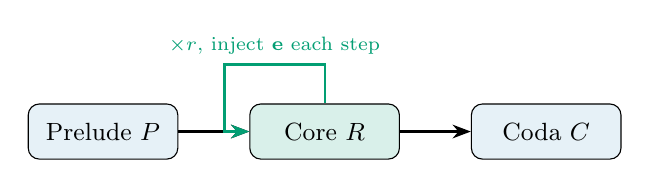
\begin{tikzpicture}[scale=0.9,
        box/.style={draw, rounded corners, minimum width=1.9cm, minimum height=0.7cm, font=\small},
        arr/.style={-{Stealth}, thick}]
        \node[box, fill=positive!10] (P) {Prelude $P$};
        \node[box, fill=emphasis!15, right=0.9cm of P] (R) {Core $R$};
        \node[box, fill=positive!10, right=0.9cm of R] (C) {Coda $C$};
        \draw[arr] (P) -- (R); \draw[arr] (R) -- (C);
        \draw[arr, emphasis, thick] (R.north) -- ++(0,0.55) -| node[pos=0.25, above, font=\scriptsize] {$\times r$, inject $\mathbf{e}$ each step} ([xshift=-0.35cm]R.north west) -- ([xshift=-0.35cm]R.west) -- (R.west);
      \end{tikzpicture}
      \end{center}
      {\small Source: Geiping et al. 2025, Fig.~2 (redrawn)}
  \end{columns}
  \textit{Takeaway: recurrence trades parameters for compute; this talk asks \HL{when that trade wins}.}
\end{frame}

\begin{frame}{Taxonomy: where the loop sits, and three orthogonal axes}
  \vspace{4pt}
  \begin{center}
  \small
  \begin{tabular}{@{}lp{0.36\textwidth}p{0.40\textwidth}@{}}
    \toprule
    Granularity & Definition & Representatives \\
    \midrule
    model-loop & whole stack fed back & UT (2018), Huginn core, Ouro \\
    block-loop & contiguous middle segment loops & Huginn 3-stage, Hyperloop, Training-Free, SMELT \\
    layer-loop & each layer repeats $K$ times, then next layer & Loopie, Training-Free layer-mode, MixerLoop \\
    latent conditioning & previous state injected as condition & Coconut, PLT (CLP), Latent Recurrent Tr. \\
    \bottomrule
  \end{tabular}
  \end{center}
  \vspace{6pt}
  \begin{columns}[T]
    \column{0.31\textwidth}
      \textbf{Loop count}\\ fixed (Loopie, LoopCoder-v2) / random-train, free-test (Huginn) / per-token halting (ACT, MoR, TaH)
    \column{0.31\textwidth}
      \textbf{Training}\\ from scratch (Huginn, Ouro, Loopie) / retrofit (Relaxed Recursive, Retrofitted Recurrence) / \HL{training-free}
    \column{0.31\textwidth}
      \textbf{What the loop is}\\ unrolled LM / fixed point (DEQ, STARS) / ODE refinement (Training-Free) / supervised latent CoT (LOTUS) / RL on steps (RLTT)
  \end{columns}
\end{frame}

% =====================================================================
\section{Five core papers}

\begin{frame}{Universal Transformers (2018): recurrence + adaptive halting}
  \begin{columns}[T]
    \column{0.55\textwidth}
      \begin{block}{Mechanism (Dehghani et al., ICLR 2019)}
        \begin{align*}
          A^t &= \mathrm{LN}\!\big(H^{t-1}{+}P^t + \mathrm{MHSA}(H^{t-1}{+}P^t)\big)\\
          H^t &= \mathrm{LN}\!\big(A^t + \mathrm{Transition}(A^t)\big)
        \end{align*}
      \end{block}
      \begin{itemize}
        \item Parameters shared over time steps $t$; coordinate embedding $P^t$ = position + time step
        \item ACT halting per position: ponder time 2.3 / 3.1 / 3.8 steps for 1 / 2 / 3 supporting facts
        \item Turing-complete given memory (reduces to Neural GPU)
      \end{itemize}
    \column{0.42\textwidth}
      \vspace{4pt}
      \begin{center}
      \small
      \begin{tabular}{@{}lrrr@{}}
        \toprule
        Task & Trans. & UT & +ACT \\
        \midrule
        bAbI 10K joint (err\%) & 22.1 & 0.47 & \textbf{0.29} \\
        LAMBADA ppl & 7321 & 319 & \textbf{142} \\
        WMT14 En-De BLEU & 28.0 & \textbf{28.9} & -- \\
        \bottomrule
      \end{tabular}
      \end{center}
      \vspace{4pt}
      \con{Open problems it left:} parameter--compute ratio, training stability, inference cost.
  \end{columns}
  \vspace{4pt}
  \textit{Takeaway: gains concentrate on hard instances; the same pattern reappears in Huginn seven years later.}
\end{frame}

\begin{frame}{Huginn-3.5B (Feb 2025): recurrent depth trained at modern scale}
  \begin{columns}[T]
    \column{0.5\textwidth}
      \begin{itemize}
        \item Shape $(2,4,2)$, $h = 5280$, 3.5B params; $r=32 \Rightarrow$ 132 effective layers
        \item Train: $r \sim$ log-normal Poisson ($\bar r=32$), \HL{backprop through last $k=8$ steps only}
        \item 800B tokens, 4096 AMD MI250X, constant LR $4\times10^{-5}$, sandwich norm
        \item Two failed runs: hidden-state collapse; recurrence collapse ($r{=}1 \equiv r{=}32$)
      \end{itemize}
      \begin{alertblock}{Fair comparison is at 0.18T tokens (Table 4)}
        Same setup, non-recurrent: ARC-E 46.42, GSM8K-CoT 2.20 \quad vs.\quad recurrent $r{=}32$: \textbf{53.62}, \textbf{10.24}
      \end{alertblock}
    \column{0.47\textwidth}
      \vspace{4pt}
      \begin{center}
      \small
      \begin{tabular}{@{}rrrrr@{}}
        \toprule
        $r$ & ARC-E & HellaSwag & MMLU & GSM8K CoT \\
        \midrule
        4  & 49.07 & 43.46 & 23.39 & -- \\
        8  & 65.11 & 58.54 & 25.29 & -- \\
        16 & 69.49 & 64.67 & 31.25 & -- \\
        \rowcolor{positive!12} 32 & \textbf{69.91} & \textbf{65.21} & \textbf{31.38} & \textbf{42.08} \\
        \bottomrule
      \end{tabular}
      \end{center}
      {\small Table 1--2; GSM8K CoT strict, with system prompt.}\\[4pt]
      \small The last 620B tokens improve $r{=}32$ but not $r{=}1$ (34.01 $\to$ 34.89): everything learned lives in the loop.
  \end{columns}
\end{frame}

\begin{frame}{Huginn: what the loop buys, and what emerges in latent space}
  \begin{columns}[T]
    \column{0.48\textwidth}
      \begin{block}{Zero-shot capabilities}
        \begin{itemize}
          \item Per-token adaptive exit (KL $< 5{\times}10^{-4}$): MT-Bench $5.63 \to 5.56$
          \item KV-cache sharing with budget 4: no loss
          \item Continuous CoT: warm-start $\mathbf{s}_0$ from previous token
          \item Self-speculative decoding without a draft model
        \end{itemize}
      \end{block}
      \begin{itemize}
        \item More context $\Rightarrow$ more loops needed: ARC-C saturates at 8 (0-shot) vs.\ 32 (25--50-shot)
        \item Open-book OBQA $+11.0$: \pos{reasons over context}, \con{memorizes little}
      \end{itemize}
    \column{0.48\textwidth}
      \begin{exampleblock}{Latent geometry (Sec.~7)}
        Fixed points for most tokens; \textbf{orbits} for numeric tokens; \textbf{sliders} (steady drift) for key tokens; path independence across $\mathbf{s}_0$.
      \end{exampleblock}
      \con{Caveats:} one run, LR never cooled; $r{=}32$ inference is $16\times$ an 8-layer model; Lu et al.\ 2025 find limited interpretable latent CoT.
  \end{columns}
  \vspace{4pt}
  \textit{Takeaway: ``3.5B behaves like 50B'' is FLOP-equivalence, not benchmark-equivalence.}
\end{frame}

\begin{frame}{Training-Free Looped Transformers (May 2026): a layer is one Euler step}
  \begin{columns}[T]
    \column{0.5\textwidth}
      \begin{block}{Insight (Chen, Li, Liang, Lao, Liu; UT Austin)}
        Pre-norm layer $L(x) = x + F(x)$ is forward Euler ($h{=}1$) on $\dot x = F(x)$.
        Naive $K$-fold looping integrates to $t{=}K$ --- \con{post-loop layers never saw that}.
        Sub-step instead:
        \[ x_{k+1} = \Big(1-\tfrac{1}{K}\Big)x_k + \tfrac{1}{K}\,g(x_k) \]
      \end{block}
      \begin{itemize}
        \item RK tableau with anchor $\beta$: output $= \beta\, g(x_0) + (1-\beta)\,F^K(x_0)$
        \item Toy net, $K{=}8$: naive MSE 335 vs.\ sub-step 1.04; accelerators (Anderson, heavy-ball, Aitken) never beat RK $\Rightarrow$ mid-stack is \HL{an ODE flow, not a contraction}
      \end{itemize}
    \column{0.47\textwidth}
      \vspace{4pt}
      \begin{center}
      \small
      \begin{tabular}{@{}llrr@{}}
        \toprule
        Model & Benchmark & Base & $\Delta$pp \\
        \midrule
        Qwen3-4B-Instruct & MMLU-Pro & 57.1 & \textbf{+2.64} \\
        Qwen3-4B-Instruct & GPQA-Main & 33.7 & \textbf{+2.01} \\
        Qwen1.5-MoE-A2.7B & ARC-C & 48.3 & \textbf{+2.30} \\
        Llama-3.2-1B-Inst. & GPQA-Main & 27.9 & +1.79 \\
        Moonlight-16B-A3B & OBQA & 31.6 & +1.20 \\
        DeepSeek-V2-Lite & ARC-C & 57.9 & +0.85 \\
        \bottomrule
      \end{tabular}
      \end{center}
      {\small One recipe, no per-cell tuning: middle 4 layers, 3-stage RK, block-mode dense / layer-mode MoE.}
  \end{columns}
\end{frame}

\begin{frame}{Training-Free: window size, depth fraction, and the MoE rule}
  \begin{columns}[T]
    \column{0.48\textwidth}
      \vspace{4pt}
      \begin{center}
      \begin{tabular}{@{}rlr@{}}
        \toprule
        Window $n$ & Layers & $\Delta$ (16-task) \\
        \midrule
        1 & [14] & +0.18 \\
        3 & [13--15] & +0.21 \\
        \rowcolor{positive!12} 4 & [12--15] & \textbf{+0.55} \\
        6 & [11--16] & \con{$-0.82$} \\
        28 & all & \con{$-27.73$} \\
        \bottomrule
      \end{tabular}
      \end{center}
      {\small Qwen3-1.7B-Base, forward Euler $K{=}2$ (Table 2a).}
    \column{0.48\textwidth}
      \begin{itemize}
        \item \textbf{Depth-fraction rule}: optimal window center at $0.43$--$0.71$ of depth ($>$1.7B), $0.25$--$0.56$ ($<$1B)
        \item \textbf{MoE needs layer-mode}: block-mode re-routes experts each iteration (routing thrash); layer-mode gates once
        \item 45 cells: 60\% positive, 27\% neutral, \HL{87\% non-negative}; failures = sub-3B distilled on knowledge MC
        \item Naive loop at $K{=}6$: $-17.71$pp; this method stable for $K \le 24$
      \end{itemize}
  \end{columns}
  \vspace{6pt}
  \textit{Takeaway: an untrained model can only be looped in a small mid-stack window; gains cap at $\sim$2--3 points.}
\end{frame}

\begin{frame}{LoopCoder-v2 (Jun 2026): in a Parallel Loop Transformer, loop 2 is almost everything}
  \begin{columns}[T]
    \column{0.46\textwidth}
      \begin{block}{PLT (Wu et al.\ 2025) flattens cost}
        \begin{itemize}
          \item Shared first-loop KV + gated sliding window ($w{=}64$): KV $O(LSd)$
          \item Cross-loop position offset: $B^{(r)} = \mathrm{Embed}(x) + \mathrm{shift}(\mathbf{h}^{(r-1)})$ $\Rightarrow$ loops run in one pass
          \item \con{Price}: token $i$ receives its neighbor's state (positional mismatch)
        \end{itemize}
      \end{block}
      7B dense, $R \in \{1,2,3,4\}$ each trained from scratch on 18T tokens; same SFT; 1M GPU hours.
    \column{0.52\textwidth}
      \vspace{4pt}
      \begin{center}
      \small
      \begin{tabular}{@{}lrrrrr@{}}
        \toprule
        7B & HE+ & LCB & SWE-V & Multi-SWE & Avg \\
        \midrule
        $R{=}1$ & 81.1 & 27.4 & 43.0 & 14.0 & 38.0 \\
        \rowcolor{positive!12} $R{=}2$ & \textbf{84.1} & \textbf{35.4} & \textbf{64.4} & \textbf{31.0} & \textbf{46.5} \\
        $R{=}3$ & 75.0 & 28.6 & 27.6 & 11.0 & 36.9 \\
        $R{=}4$ & 76.8 & 24.5 & 22.4 & 9.3 & 34.3 \\
        \bottomrule
      \end{tabular}
      \end{center}
      {\small Table 2. $R{=}2$ on SWE-bench Verified (64.4) beats Kimi-Dev-72B (60.4) and Qwen3-235B-A22B (45.2).}
  \end{columns}
  \vspace{4pt}
  \textit{Takeaway: strongly non-monotonic in $R$ --- the next slide shows why.}
\end{frame}

\begin{frame}{LoopCoder-v2: gain--cost scissors, and CoT $+$ loop is super-additive}
  \begin{columns}[T]
    \column{0.5\textwidth}
      \vspace{4pt}
      \begin{center}
      \begin{tabular}{@{}lrrrr@{}}
        \toprule
        Loop & $\delta^{(r)}$ & $\Delta p^{(r)}$ & eff.\ rank & $\cos\theta$ \\
        \midrule
        \rowcolor{positive!12} $r{=}2$ & \textbf{846} & \textbf{1.75} & \textbf{174.6} & $-0.72$ \\
        $r{=}3$ & 464 & 1.32 & 172.5 & $-0.46$ \\
        $r{=}4$ & 1014 & 1.58 & 158.2 & 0.04 \\
        \bottomrule
      \end{tabular}
      \end{center}
      {\small PLT4, 500 samples (Table 3). Offset cost $\Omega^{(r)} = \frac1S\sum_i\|\mathbf{h}_i^{(r-1)} - \mathbf{h}_{i-1}^{(r-1)}\|$ is $\approx$ constant.}
      \begin{itemize}
        \item Effective rank peaks at loop 2, then \con{narrows}
        \item Updates oscillate ($\cos\theta<0$); attention routing freezes after loop 2
        \item Fixed offset tax is \textbf{30--45$\times$} the marginal gain from loop 3 on
      \end{itemize}
    \column{0.46\textwidth}
      \begin{exampleblock}{Thinking mode on top of $R{=}2$ (Table 4)}
        \begin{center}
        \begin{tabular}{@{}lrr@{}}
          \toprule
           & Instruct & Thinking \\
          \midrule
          LiveCodeBench & 35.4 & \textbf{62.3} \\
          CRUX & 86.9 & \textbf{93.5} \\
          MultiPL-E & 73.9 & \textbf{77.8} \\
          \bottomrule
        \end{tabular}
        \end{center}
        Explicit CoT alone does not help the non-looped model; loop alone gives single digits. Together: \HL{super-additive}.
      \end{exampleblock}
      \con{Scope:} ``two is optimal'' is a PLT property (CLP tax). Huginn improves monotonically to $r{=}32$.
  \end{columns}
\end{frame}

\begin{frame}{Loop the Loopies! (Jul 2026): the first compute-matched win}
  \begin{columns}[T]
    \column{0.5\textwidth}
      \begin{block}{Loopie Recipe (match by measured step time)}
        \begin{enumerate}
          \item Halve stored layers, loop twice: $LR$ unchanged, activation memory $\propto sbDL$ halves
          \item Spend memory on $2\times$ micro-batch (tokens/step unchanged)
          \item Reinvest measured speed-up into width; pick equal wall-clock step time
        \end{enumerate}
      \end{block}
      \begin{center}
      \small
      \begin{tabular}{@{}lrrrrr@{}}
        \toprule
        Config & $D$ & $L$ & $R$ & $\hat C$ & $\hat M_{\mathrm{act}}$ \\
        \midrule
        Qwen3-30B-A3B ref. & 2048 & 48 & 1 & 1.00 & 1.00 \\
        seed Loopie & 2048 & 24 & 2 & 1.00 & 0.50 \\
        \rowcolor{positive!12} \textbf{Loopie-20B-A2B} & 2304 & 27 & 2 & \textbf{1.42} & 0.63 \\
        \bottomrule
      \end{tabular}
      \end{center}
    \column{0.46\textwidth}
      \begin{itemize}
        \item \textbf{Layer-loop} ($L_1L_1L_2L_2\dots$) overtakes model-loop after $\sim$1.2T tokens; pipeline-parallel friendly
        \item Compute-matched run: overtakes reproduced Qwen3-30B-A3B after \HL{$\sim$600B of 800B tokens}
        \item Scaling ladder 0.15B--1B active params: Loopie wins all 4 rungs, gap does not shrink
        \item Why $R{=}2$: marginal return of $N\times$ loops vs.\ $N\times$ layers decays fastest after 2
      \end{itemize}
      \con{Accounting:} nominal FLOPs $+42\%$; inference does 54 vs.\ 48 block passes per token; no latency reported.
  \end{columns}
\end{frame}

\begin{frame}{Loopie: post-training with supervised pre-training (SPT) and RL}
  \begin{columns}[T]
    \column{0.42\textwidth}
      \begin{block}{SPT = SFT loss mask $+$ pre-training scale}
        Loss on target tokens only; global batch $\ge$1024, sequence $\ge$128K, $\ge$128M token positions per batch, 2T tokens, 10 epochs.\\
        \pos{Pretraining metrics $\uparrow$} and \pos{reasoning metrics $\uparrow$}; no overfitting, no forgetting.
      \end{block}
      RL: GSPO (sequence-level ratio/clip) + DAPO clip-higher and dynamic sampling; math then code; 32K $\to$ 64K.
    \column{0.54\textwidth}
      \vspace{4pt}
      \begin{center}
      \footnotesize
      \begin{tabular}{@{}lrrr@{}}
        \toprule
         & Qwen3 & Nemotron & \textbf{Loopie} \\
         & 30B-A3B (36T) & 3 Nano (25T) & \textbf{20B-A2B (3.5T)} \\
        \midrule
        MMLU & 85.83 & 80.52 & \textbf{81.28} \\
        ARC-C & 96.67 & 91.96 & 93.52 \\
        BBH & 86.59 & 68.76 & 82.28 \\
        IFEval & 85.58 & 77.05 & 84.72 \\
        AIME 24 & 90.10 & 85.00 & \textbf{92.09} \\
        AMC & 96.73 & 91.80 & 94.21 \\
        \bottomrule
      \end{tabular}
      \end{center}
      {\small Table 3. Loopie-6B-A0.6B Thinking: AIME24 80.42, AIME25 70.83 (Ouro-2.6B: 62.50 / 51.67).}
  \end{columns}
  \vspace{4pt}
  \textit{Takeaway: under one-seventh of the pretraining tokens, a looped MoE matches 25T-token peers on knowledge benchmarks.}
\end{frame}

% =====================================================================
\section{The wider map, ten insights, and what changed since September}

\begin{frame}{The 2026 literature: ten themes, roughly sixty papers}
  \vspace{4pt}
  \begin{center}
  \footnotesize
  \begin{tabular}{@{}lp{0.74\textwidth}@{}}
    \toprule
    Theme & Representative results \\
    \midrule
    Theory & $k$ layers looped $L$ times $\approx kL$ layers (Saunshi 25); loops vs.\ CoT separation (Xu \& Sato 25); budget law $v \approx n/T$ (Zhang 26) \\
    Scaled pretraining & Huginn 3.5B/0.8T, Ouro 2.6B/7.7T, LoopCoder-v2 7B/18T, Loopie 20B-A2B/3.5T, Nanbeige4.2-3B/28T, SMELT to 54B; loop counts 2--4 \\
    Efficiency & PLT (latency), diffusion-style sampler $5\times$, MELT constant KV, Looped Latent Attention $32\times$ KV, LT2 linear attention, LoopQ \\
    Stability & residual scaling $\varepsilon{=}1/N$ (not $1/\sqrt L$), DeepLoop exponent $1/4 \to 1/2$, STARS spectral radius, settling/drifting regimes \\
    Adaptive halting & MoR (NeurIPS 25), Think-at-Hard (skip 93\% of tokens), LoopFormer, RecurTrace (2.0 loops avg.) \\
    Retrofit / training-free & Relaxed Recursive (LoRA), Retrofitted Recurrence, Training-Free RK, Program-of-Layers (ICML 26) \\
    Post-training & RLTT trajectory credit $+10.9\%$, LoopRPT, LOTUS latent CoT matches explicit at 3B, SPT \\
    Interpretability & orbits/sliders (Huginn), limited latent-CoT evidence (Lu 25), Jacobian lens: Ouro rebuilds workspace per loop \\
    Tiny reasoners & HRM 27M, TRM 7M (ARC-AGI-1 45\%), Attractor Models, Denoising Recursion \\
    Applications & LoopViT (ARC 65.8\% at 18M), RD-VLA ($0\% \to 90\%$, $80\times$ faster), compositional tool calling, agentic products \\
    \bottomrule
  \end{tabular}
  \end{center}
\end{frame}

\begin{frame}{Insights 1--3: narrow win, two regimes, converging on the middle}
  \begin{enumerate}
    \item \textbf{Compute-matched wins exist, through a narrow door.} Loopie (step time) and SMELT (FLOPs/params/KV, $6.8$--$18\%$ savings) win only with \HL{MoE $+$ layer/mid-stack loop $+$ two loops}. One recurrence is worth $r^{0.46}$ unique parameters ($0.38$ under truncated backprop): loops cannot replace parameters; Loopie converts \emph{activation memory} into width.
    \item \textbf{``How many loops'' splits by where compute binds.} Fixed pretraining budget $\Rightarrow R{=}2$ (Loopie, LoopCoder-v2, SMELT, Nanbeige). Variable inference compute $\Rightarrow$ adaptive and deep (Huginn: 8 loops zero-shot, 32 with 25--50 shots). ``Three regress'' is \con{PLT's positional tax}.
    \item \textbf{Granularity shrinks, placement converges.} Whole model $\to$ three-stage $\to$ per-layer / mid-stack $\to$ mixer-only (MixerLoop: 41.5\% of gain at $-45.9\%$ looped FLOPs). Optimal window center $\approx 0.5$ of depth; MoE needs layer-mode (two independent papers agree).
  \end{enumerate}
\end{frame}

\begin{frame}{Insights 4--7: ODE vs.\ fixed point, stability theorems, inference cost, CoT complementarity}
  \begin{enumerate}\setcounter{enumi}{3}
    \item \textbf{Two philosophies.} Training-Free: a pretrained mid-stack is an \pos{ODE flow} (sub-step, keep the endpoint). STARS / Fixed-Point Reasoners / Attractor Models: \emph{train} the loop to be a \pos{fixed point}. Viakhirev et al.: settling operators are depth-safe; Huginn is non-settling; LoopCoder-v2's $\cos\theta<0$ is drift.
    \item \textbf{Stability went from folklore to theorems.} $\varepsilon{=}1/N$ residual scaling; DeepNorm exponent $1/2$; LR depends only on unique layers and transfers across $N$; stable training to 12--15 loops.
    \item \textbf{Inference cost decomposes into three stackable fixes.} Latency (PLT, diffusion sampler $5\times$), KV (sharing; LLA low-rank $32\times$), quantization (LoopQ). \con{Matched training compute $\ne$ matched inference cost.}
    \item \textbf{Loops and CoT are complements.} LoopCoder-v2 LCB $+26.9$ super-additive; LOTUS matches explicit CoT at 3B with $2.5$--$6.9\times$ lower thought latency. Standard GRPO credits only the final latent state: RLTT ($+10.9\%$) and LoopRPT redesign credit assignment.
  \end{enumerate}
\end{frame}

\begin{frame}{Insights 8--10: capability profile, applications, productization}
  \begin{enumerate}\setcounter{enumi}{7}
    \item \textbf{Loops manipulate knowledge; they do not store it.} Ouro attributes gains to knowledge manipulation; Huginn open-book $+11.0$; Frey et al.: loops help math, memory banks help commonsense; Dual-Path gates send arithmetic tokens ``deep'' and function words ``wide''. Best partners: \HL{retrieval, long context, MoE expert banks}.
    \item \textbf{From puzzles to agents and embodiment.} SWE-bench Verified $+21.4$ (LoopCoder-v2); compositional tool calling improves with depth; Nanbeige4.2-3B beats Qwen3.5-9B on agentic benchmarks; RD-VLA $0\% \to 90\%$ with four iterations, $80\times$ faster than token-reasoning VLAs.
    \item \textbf{Productization started; tooling lags.} Five open families (Huginn, Ouro, LoopCoder-v2, Loopie, Nanbeige4.2-3B). Nanbeige4.2-3B ships with five out-of-the-box bugs in HF transformers and $2\times$ attention memory from layer reuse. No standard interface yet for looped inference, KV, or quantization.
  \end{enumerate}
\end{frame}

\begin{frame}{What changed since September 2026}
  \noindent{\footnotesize 211 papers added on 2026-11-06: 167 first submitted 2026-09-01 to 2026-11-06, plus 44 June--August papers the first search missed.\par}
  \begin{center}
  \footnotesize\setlength{\tabcolsep}{4pt}
  \begin{tabular}{@{}r>{\raggedright\arraybackslash}p{0.30\textwidth}>{\raggedright\arraybackslash}p{0.37\textwidth}l>{\raggedright\arraybackslash}p{0.10\textwidth}@{}}
    \toprule
    \# & Change & Key number (conditions) & arXiv & Insight \\
    \midrule
    1 & \textbf{From-scratch loops beat matched baselines without MoE}; retrofitting is a mixed bet & Loopback: lower loss with \textbf{40--75\%} of the Transformer parameters (matched tokens, executed depth) & 2611.07226 & \pos{refines 1} \\
    2 & \textbf{Two loops is the optimum of current designs, not a rule} & LOOM 700M: best at \textbf{5 loops}, near-iso-FLOPs & 2610.01153 & \con{revises 2} \\
    3 & \textbf{Serving is the largest cluster}; looped models run in production engines & LoopVQ in SGLang: up to \textbf{6.1$\times$} Ouro serving throughput & 2611.05304 & \con{revises 10}; \pos{refines 6} \\
    4 & \textbf{Loop depth changes safety behaviour} & Ouro-1.4B-Thinking, half depth: harmful-help rate up \textbf{5.3$\times$}, 89\% of GSM8K accuracy kept & 2610.15218 & \HL{new}; cf.\ 7 \\
    5 & \textbf{``Manipulate, not store'' becomes architecture} & Fact edits propagate \textbf{0.71--0.96} with memory vs.\ 0.04--0.30 with loops alone (synthetic) & 2606.20737 & \pos{supports 8} \\
    6 & \textbf{Applications reach generative and scientific models} & 260M Looped-DiT beats a 6.5$\times$ larger text-to-image model at \textbf{4.9$\times$} lower inference compute & 2609.40305 & \pos{extends 9} \\
    \bottomrule
  \end{tabular}
  \end{center}
  \textit{Takeaway: insight 2 and the toolchain half of 10 are revised; post-training must cover every depth.}
\end{frame}

\begin{frame}{Five circulation errors, checked against the papers}
  \vspace{4pt}
  \begin{center}
  \small
  \begin{tabular}{@{}p{0.42\textwidth}p{0.54\textwidth}@{}}
    \toprule
    Common claim & What the paper says \\
    \midrule
    Huginn crushes its baseline ``at the same 0.8T tokens'' & Baseline trained 0.18T; at 0.18T recurrent ARC-E 53.62 vs.\ 46.42 (Table 4) \\
    ``Two loops suffice, three regress'' is a law & PLT-specific (CLP tax), each $R$ trained separately; Huginn monotone to $r{=}32$ \\
    Loopie and Qwen3-30B-A3B use ``the same compute'' & Same measured step time; nominal FLOPs $+42\%$; inference cost unreported; reference is an 800B-token reproduction \\
    Training-Free makes open models ``stronger'' & $+1$--$2.6$pp on knowledge MC; sub-3B distilled models can lose; $+15$--$30\%$ latency \\
    Huginn ``performs like 50B at 3.5B'' & FLOP-equivalent; on benchmarks near OLMo-7B, behind OLMo-2-7B \\
    \bottomrule
  \end{tabular}
  \end{center}
\end{frame}

\begin{frame}{GPT-6 Astra: what is verifiable and what is inference}
  \begin{alertblock}{Not verifiable here}
    Which loop Astra uses, how many, how trained. OpenAI's page discloses no architecture; The Information's report is anonymously sourced; neither was accessible to us.
  \end{alertblock}
  \begin{itemize}
    \item \textbf{Inference 1.} The public recipe closest to ``frontier scale $+$ compute-matched'' is Loopie/SMELT: MoE, mid-stack or per-layer, small loop count.
    \item \textbf{Inference 2.} ``OpenAI beat two-loop saturation'' starts from a false premise --- saturation is PLT-specific; the real bottleneck is inference cost, already cut $\sim$10$\times$ by public KV compression and parallel sampling.
    \item \textbf{Inference 3.} Reported ``security concerns'' match a real gap: latent reasoning has no readable intermediate tokens; probes depend on layer and decoding method.
    \item \textbf{Inference 4.} Loopie (Jul), LLA (Jul), SMELT (1 Sep), Astra (early Sep): several groups reached usability simultaneously.
  \end{itemize}
\end{frame}

% =====================================================================
\section{Open problems and takeaways}

\begin{frame}{Open problems}
  \begin{columns}[T]
    \column{0.48\textwidth}
      \begin{enumerate}
        \item Compute-matched evidence for $R \ge 4$ (all wins are at $R{=}2$)
        \item The full inference bill: step time $+$ latency $+$ peak KV in one paper
        \item Scaling-law form at 100B$+$ (SMELT to 54B, Schwethelm to $\sim$1B)
        \item Adaptive halting beyond 8B (only Ouro's entropy allocation at 7.7T)
      \end{enumerate}
    \column{0.48\textwidth}
      \begin{enumerate}\setcounter{enumi}{4}
        \item Supervisability of latent reasoning without gold CoT (safety)
        \item Mechanism of layer-loop (only SMELT's attention-sink account)
        \item Loops vs.\ sequence-length scaling (Hidden Decoding, WeLM 617B) at 100B$+$
      \end{enumerate}
      \begin{exampleblock}{Most valuable gaps}
        Compute-matched scaling laws at $R \ge 4$; loop-specific RL objectives with trajectory-level credit.
      \end{exampleblock}
  \end{columns}
\end{frame}

\begin{frame}{Three takeaways}
  \begin{enumerate}
    \item \textbf{Recurrent depth passed the compute-matching gate in 2026} --- via layer-loop, MoE, and two loops, with the win coming from activation memory, not from loops replacing parameters.
    \item \textbf{Pick the loop count by where compute binds}: 2 for frontier pretraining; adaptive and deep when inference compute is variable. Two-loop saturation is PLT's price, not a ceiling.
    \item \textbf{Loop under CoT, not instead of it}; redesign RL credit for latent trajectories; measure latency and KV before shipping.
  \end{enumerate}
  \vspace{8pt}
  \begin{block}{Practical recipe}
    Zero-training: middle 4 layers, 3-stage RK, $\beta$ mid, layer-mode on MoE. \quad
    From scratch: MoE, layer-loop, $R{=}2$, match by measured step time, $1/N$ residual scaling, SPT $+$ trajectory RL. \quad
    Variable inference: sequential loop, random-$r$ training, truncated backprop, adaptive exit, KV codec.
  \end{block}
\end{frame}

\begin{frame}[allowframebreaks]{References}
  \small
  \begin{thebibliography}{9}
    \bibitem{ut} M. Dehghani, S. Gouws, O. Vinyals, J. Uszkoreit, \L. Kaiser. Universal Transformers. ICLR 2019. arXiv:1807.03819.
    \bibitem{huginn} J. Geiping, S. McLeish, N. Jain, J. Kirchenbauer, S. Singh, B. Bartoldson, B. Kailkhura, A. Bhatele, T. Goldstein. Scaling up Test-Time Compute with Latent Reasoning: A Recurrent Depth Approach. arXiv:2502.05171, 2025.
    \bibitem{tf} L. Chen, J. Li, C. Liang, N. Lao, Q. Liu. Training-Free Looped Transformers. arXiv:2605.23872, 2026.
    \bibitem{lc2} J. Yang et al. LoopCoder-v2: Only Loop Once for Efficient Test-Time Computation Scaling. arXiv:2606.18023, 2026.
    \bibitem{loopie} Z. Gao, Y. Chen, Y. Xiao, X. Yang, R. Tao, J. Zhou, B. Dai. Loop the Loopies! arXiv:2607.16051, 2026.
    \bibitem{smelt} S. Wang et al. SMELT: Scaling Laws for Compute-Matched MoE Looped Transformers. arXiv:2609.01343, 2026.
    \bibitem{plt} B. Wu et al. Parallel Loop Transformer for Efficient Test-Time Computation Scaling. arXiv:2510.24824, 2025.
    \bibitem{ouro} R.-J. Zhu et al. Scaling Latent Reasoning via Looped Language Models (Ouro). arXiv:2510.25741, 2025.
    \bibitem{iso} K. Schwethelm, D. Rueckert, G. Kaissis. How Much Is One Recurrence Worth? Iso-Depth Scaling Laws for Looped Language Models. arXiv:2604.21106, 2026.
    \bibitem{lla} J. O'Neill, F. Reid. Looped Latent Attention: Cross-Loop KV Compression for Looped Transformers. arXiv:2607.15456, 2026.
    \bibitem{lotus} Y. Fan, A. Svete, K. Lee. Bridging the Gap Between Latent and Explicit Reasoning with Looped Transformers (LOTUS). arXiv:2606.31779, 2026.
    \bibitem{rltt} J. Williams, E. Tureci. Rewarding Latent Thought Trajectories Improves Reasoning in Looped Language Models. ICML 2026. arXiv:2602.10520.
  \end{thebibliography}
\end{frame}

\begin{frame}
  \centering
  {\Large Thank you}\\[10pt]
  {\small Full reports (ZH/EN), translated PDFs, HTML deck and paper list:}\\
  \url{https://github.com/asimfish/awesome_loop_transformer}
\end{frame}

% =====================================================================
\appendix
\begin{frame}{Backup Slides}\end{frame}

\begin{frame}{Backup: Huginn training details}
  \begin{itemize}
    \item Data: 800B tokens (795B realized), public, skewed to code/math; instruction data mixed into pretraining; vocab 65536; sequence 4096
    \item Hardware: ORNL Frontier, 4096 MI250X, 21 segments $\le$12h; 108.75 TFLOP/s per node (87\% achievable), 52--64 TFLOP/s per GPU at scale; data parallel + optimizer sharding only
    \item Optimizer: Adam (0.9, 0.95), constant LR $4\times10^{-5}$ after 4096 warm-up steps, no decay; locked-step sampling of $r$ per micro-batch
    \item Init: Takase et al.\ 2024, variance $2/(5h)$; output projections $1/(5hl)$ with $l = 132$
    \item Norm: four RMSNorms per layer (``sandwich''); RoPE base 50000; gated SiLU MLP; QK biases
    \item EMA over last 75 checkpoints: GSM8K flexible 47.23\% at $r{=}64$
  \end{itemize}
\end{frame}

\begin{frame}{Backup: Training-Free RK tableau and cost}
  \[ h=1,\; s=K,\; a_{ij} = \tfrac{1}{K}\,\mathbb{I}(j<i),\qquad b_1 = \beta + \tfrac{1-\beta}{K},\; b_i = \tfrac{1-\beta}{K}\ (i\ge2) \]
  \[ x_1 = x_0 + \sum_{i=1}^{K} b_i k_i = \beta\, g(x_0) + (1-\beta)\, F^{K}(x_0),\qquad F(x) = x + \tfrac{1}{K}F_g(x) \]
  \begin{itemize}
    \item Extra cost: $(b-a+1)(K-1)$ layer forwards; $K{=}3$ on a 4-layer window $\approx$ 8 extra layers ($15$--$30\%$ latency on 28--48-layer models)
    \item Seven strategies compared: naive, forward Euler, midpoint/Heun, RK4, heavy-ball, Anderson, Aitken, Uniform Loop
    \item Leakage-free transfer to Qwen3-30B-A3B at window $[22,24]$: 8 of 9 benchmarks improve (CSQA $+1.14$, MMLU-flex $+0.79$)
  \end{itemize}
\end{frame}

\begin{frame}{Backup: Loopie pretraining and RL details}
  \begin{itemize}
    \item Stage 1: Nemotron-CC-v2-HQ, $\sim$570B unique tokens, 4 epochs (2.28T); Stage 2: 1.26T annealing (SFT-v1 27.8\%, Specialized-v1 21.9\%, Code-v2 20.7\%, HQ-Synthetic 15.6\%, Math-v1 10.0\%)
    \item Qwen3 tokenizer; AdamW $\epsilon{=}10^{-15}$, wd 0.1, LR $5\times10^{-4}$ (6B) / $3\times10^{-4}$ (20B), warm-up-stable, batch 1024 $\times$ 8192
    \item Init: embeddings $\mathcal N(0, d^{-1})$; block parameters SmallInit $\mathcal N(0, 2/(5d))$
    \item RL: GSPO sequence-level ratio $s_i(\theta) = (\pi_\theta/\pi_{\theta_{\text{old}}})^{1/|o_i|}$ with asymmetric clipping; prompt-level dynamic filtering; Guru-RL math and code pools; 32K then 64K response length
    \item Code released as megatron-loopie and vllm-loopie forks
  \end{itemize}
\end{frame}

\end{document}
